\section{Analysis}
\label{sec:analysis}

\begin{takeaway}
% \textbf{Phenomenon}: 
Models are highly sensitive to increasing constraint burden.
\end{takeaway}

\paragraph{Model planning quality declines as total constraint complexity increases.}
To study how models respond to increasingly complex requirements, we construct three environment profiles, $\mathcal{E}_{low}$, $\mathcal{E}_{mid}$, and $\mathcal{E}_{high}$, by iteratively aggregating and validating world and user constraints (details in Section~\ref{sec:data-construction}). 
According to Figure~\ref{fig:analysis-iteration-bar}, both accuracy and valid plan rate exhibit a clear downward trend as the environment profile becomes more constrained across these settings.
This trend suggests that increasing constraint complexity degrades plan quality, making it harder for models both to reach the correct final answer and to maintain a valid plan throughout the interaction.

% \begin{figure*}[t]
% \centering
%     \begin{minipage}{0.5\textwidth}
%         \centering
%         \includegraphics[width=\textwidth]{figures/accuracy_iterationbar.pdf}
%     \end{minipage}%
%     \hfill
%     \begin{minipage}{0.5\textwidth}
%         \centering
%         \includegraphics[width=\textwidth]{figures/valid_plan_rate_iterationbar_normalize.pdf}
%     \end{minipage}
%     \vspace{-0.12in}
%     \caption{Model performance under increasing constraint burden. Performance drops steadily as the environment profile becomes more constrained, suggesting that current models are highly sensitive to growing dual-constraint complexity.}
%     \label{fig:analysis-iteration-bar}
%     \vspace{-0.1in}
% \end{figure*}

\begin{figure*}[t]
    % \vspace{-0.5in}
    \centering
    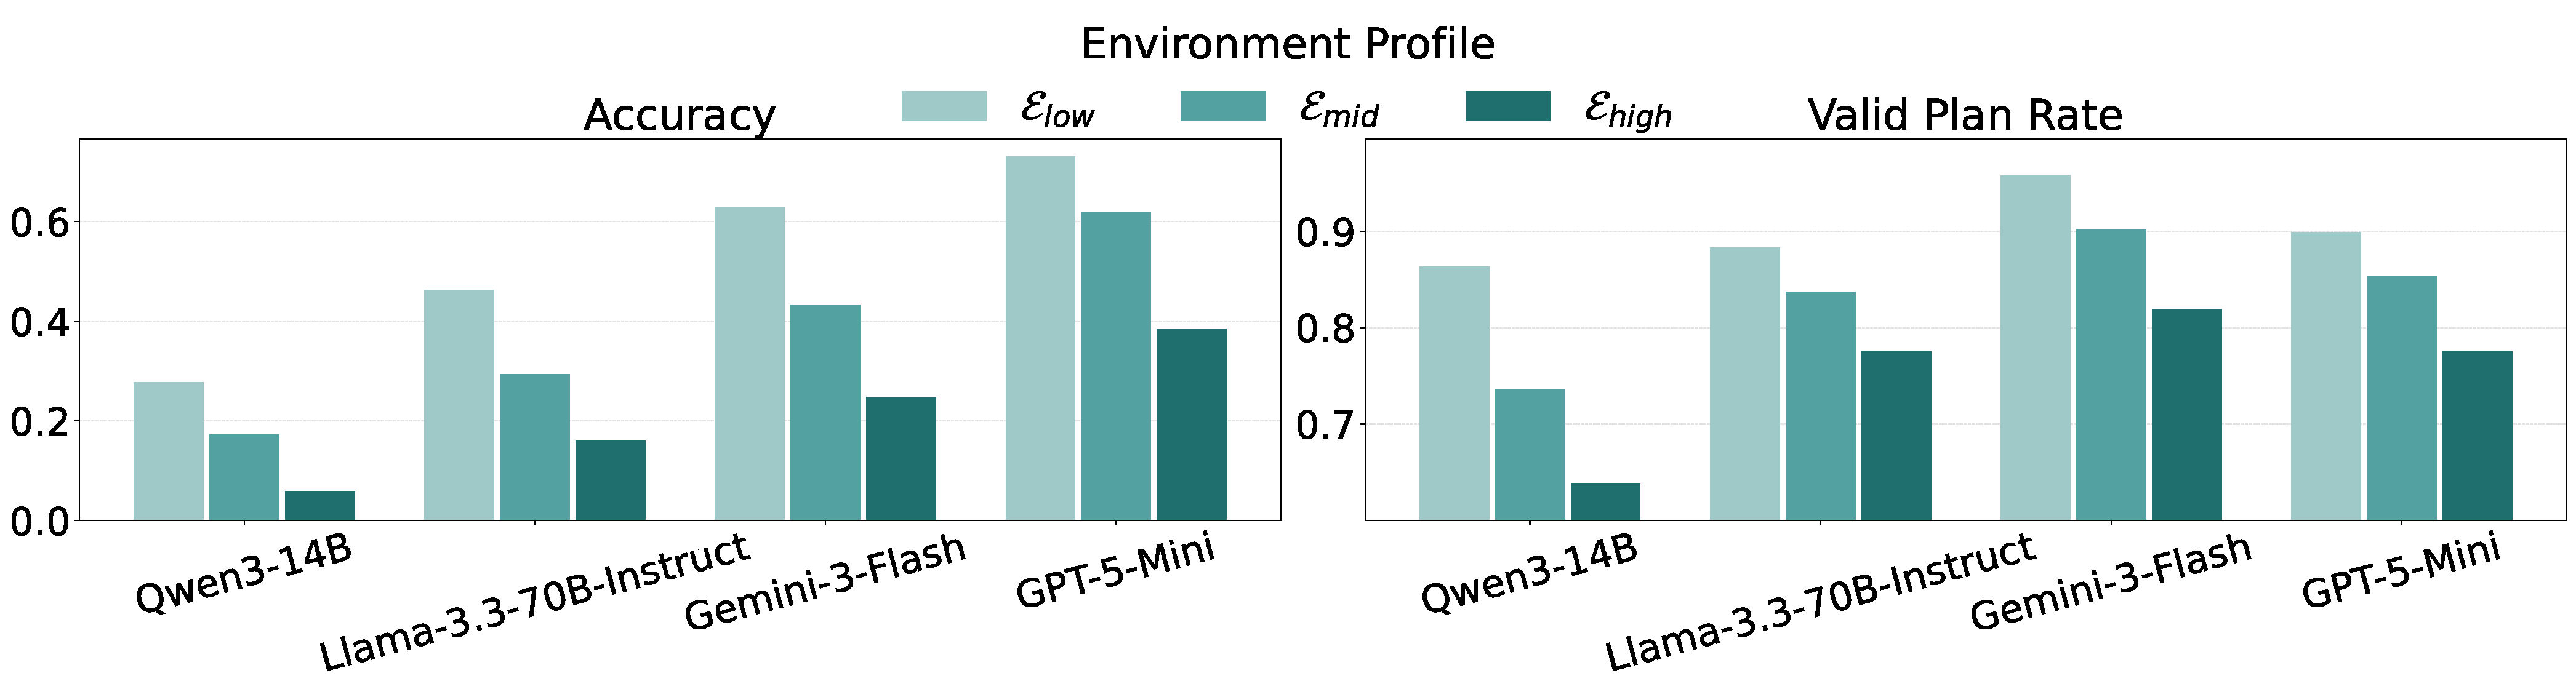
\includegraphics[width=\linewidth]{figures/accuracy_valid_plan_rate_iterationbar.pdf}
    \vspace{-0.25in}
    \caption{Model performance under increasing constraint burden. Performance drops steadily as the environment profile becomes more constrained, suggesting that current models are highly sensitive to growing dual-constraint complexity. }
    \label{fig:analysis-iteration-bar}
    \vspace{-0.1in}
\end{figure*}

\paragraph{Models' performance deteriorates as progressively disclosed constraints accumulate within a trajectory.}

\begin{figure*}[t]
    \centering
    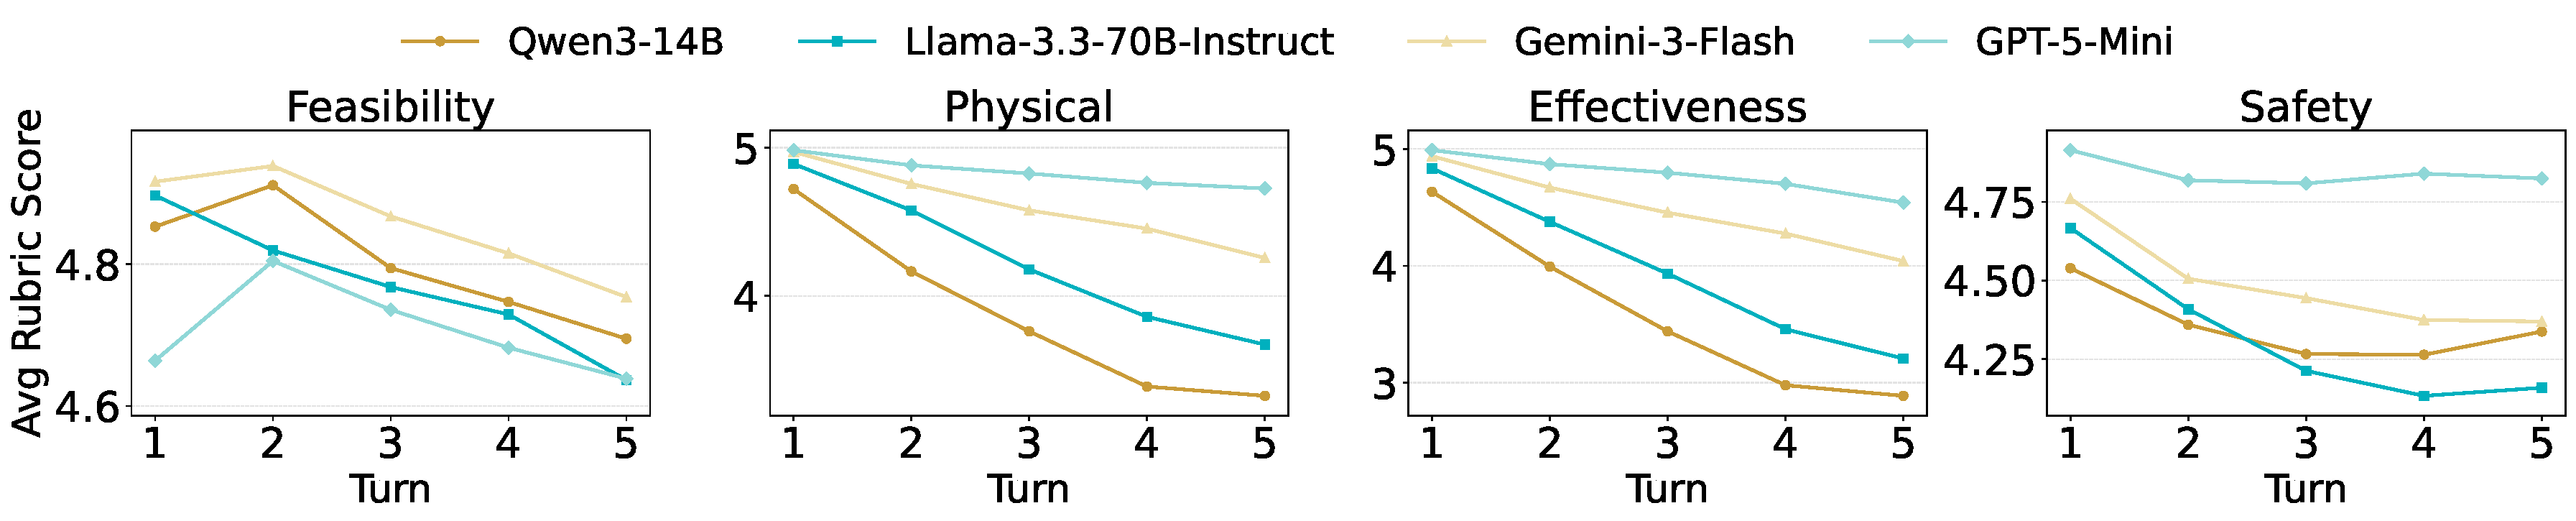
\includegraphics[width=\linewidth]{figures/turn_wise_analysis_normalized.pdf}
    \vspace{-0.25in}
    \caption{Selected model rubric scores across interaction turns under $\mathcal{E}_{mid}$. Performance deteriorates as progressively disclosed constraints accumulate within a trajectory, indicating that models struggle to maintain stable planning quality over interactions.}
    \label{fig:analysis-turnwise}
    \vspace{-0.2in}
\end{figure*}

Beyond final-task success, an important question is whether model performance remains stable as additional constraints are revealed over the course of interaction. To examine this, we conduct a turn-wise rubric analysis that aligns trajectories by turn and tracks the average score of each model on four planning dimensions as progressively disclosed constraints accumulate. As shown in Figure~\ref{fig:analysis-turnwise}, performance generally declines over time across most dimensions, with pronounced drops in the selected metrics. This trend suggests that models struggle to maintain coherent and constraint-consistent planning once they must continuously incorporate newly revealed requirements into an existing plan. The degradation is substantially milder for stronger models, which remain comparatively stable on several dimensions, but the overall pattern is consistent: progressively disclosed constraints impose a growing burden on planning quality as the trajectory unfolds.



% \begin{figure*}[t]
% \centering
%     \begin{minipage}{0.5\textwidth}
%         \centering
%         \includegraphics[width=\textwidth]{figures/accuracy_memorybar.pdf}
%     \end{minipage}%
%     \hfill
%     \begin{minipage}{0.5\textwidth}
%         \centering
%         \includegraphics[width=\textwidth]{figures/valid_plan_rate_memorybar_normalize.pdf}
%     \end{minipage}
%     \vspace{-0.12in}
%     \caption{Model performance with additional constraint tracking module. Explicitly providing previously disclosed constraints brings only limited improvement, suggesting that simple memory support is insufficient to recover robust re-planning ability.}
%     \label{fig:analysis-memory}
%     \vspace{-0.1in}
% \end{figure*}

\begin{figure*}[t]
% \vspace{-0.5in}
    \centering
    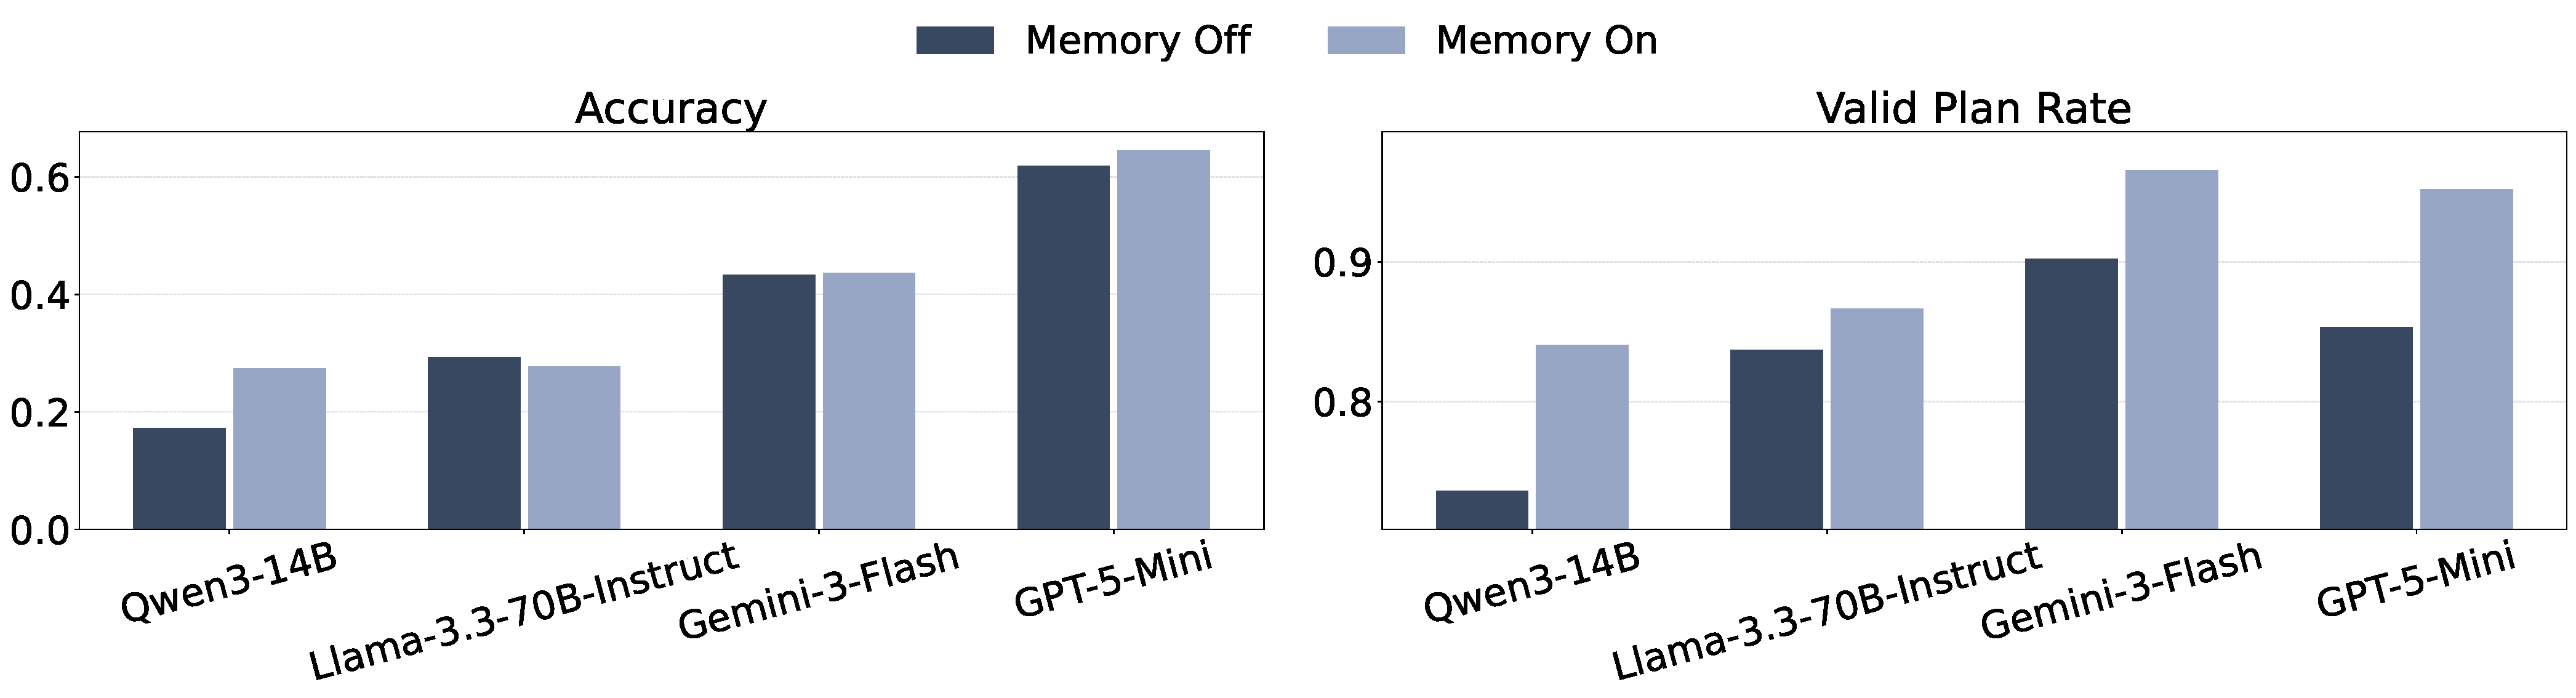
\includegraphics[width=\linewidth]{figures/accuracy_valid_plan_rate_memorybar.pdf}
    \vspace{-0.25in}
    \caption{Model performance under $\mathcal{E}_{mid}$ with additional constraint tracking module. Explicitly providing prior disclosed constraints brings only limited improvement on accuracy.}
    \label{fig:analysis-memory}
    \vspace{-0.15in}
\end{figure*}



\begin{takeaway}
\label{sec:diagnosis-analysis}
Model degradation is only partially mitigated by explicit constraint tracking and rubric feedback, while failures remain especially pronounced under user constraints.
\end{takeaway}





\begin{wraptable}{t}{0.55\columnwidth}
% \vspace{-0.3in}
\centering
\small
\setlength{\tabcolsep}{2pt}
\setlength{\extrarowheight}{2pt}
\resizebox{\linewidth}{!}{
\begin{tabular}{lcccc}
\toprule
Model & Feasibility & Physical & Effectiveness & Safety \\
\midrule
Qwen3-8B & 4.758 & 3.478 & 2.956 & 4.446 \\
Qwen3-14B & 4.755 & 3.520 & 3.030 & 4.430 \\
Qwen3-32B & \textbf{4.785} & 3.500 & 3.087 & 4.454 \\
Llama-3.3-70B-Instruct & 4.729 & 3.815 & 3.236 & 4.410 \\
DeepSeek-v4-Flash & \underline{4.771} & 4.216 & 3.868 & 4.537 \\
Gemini-3-Flash & 4.760 & 4.276 & 4.004 & 4.457 \\
Gemini-3.1-Pro & 4.628 & 4.262 & 4.055 & 4.445 \\
GPT-5 & 4.550 & \textbf{4.685} & \textbf{4.570} & \underline{4.824} \\
GPT-5-Mini & 4.615 & \underline{4.622} & \underline{4.370} & \textbf{4.828} \\
GPT-5-Nano & 4.559 & 4.428 & 3.970 & 4.810 \\
\midrule
Average & 4.691 & 4.080 & 3.715 & 4.564 \\
\bottomrule
\end{tabular}
}
\caption{Models' performance under $\mathcal{E}_{mid}$ on four major rubric dimensions.
% See Appendix~\ref{app:full-rubric-scores} for the results of remaining rubrics.
}
\label{tab:turnwise-final-selected}
\vspace{-0.15in}
\end{wraptable}

\paragraph{Instant constraint tracking module improves validity without recovering accuracy.}
As shown in the constraint failure analysis in Table~\ref{tab:main_table_2}, models often violate constraints that had already been disclosed and satisfied in earlier turns. 
This raises a natural diagnostic question: does the degradation primarily stem from failures to retain previously revealed constraints, or from difficulty constructing effective plans even when those constraints are available?
To probe this issue, we conduct an intervention in which all previously disclosed constraints are explicitly appended to the model input at every turn (details in Appendix~\ref{app:memory-analysis-details}). As shown in Figure~\ref{fig:analysis-memory}, this intervention yields only a marginal improvement in accuracy (less than 3\% for 3 out of 4 models), while producing a more noticeable gain in VPR, typically on the order of 5\%--15\%. 
These results suggest that explicit access to prior constraints helps improve constraint validity, but brings little benefit to final task success. 
Constraint tracking therefore alleviates the problem only partially.

\paragraph{Rubric-based feedback yields limited gains and destabilizes plans.}

% \begin{figure*}[t]
% \centering
%     \begin{minipage}{0.5\textwidth}
%         \centering
%         \includegraphics[width=\textwidth]{figures/accuracy_refinednewx.pdf}
%     \end{minipage}%
%     \hfill
%     \begin{minipage}{0.5\textwidth}
%         \centering
%         \includegraphics[width=\textwidth]{figures/valid_plan_rate_refinednewx.pdf}
%     \end{minipage}
%     \vspace{-0.12in}
%     \caption{Model performance with rubric-based refinement. Additional feedback yields only modest recovery and often destabilizes planning, indicating limited benefit from simple refinement signals.}
%     \label{fig:analysis-rubrics-refinement}
%     \vspace{-0.1in}
% \end{figure*}

\begin{figure*}[t]
% \vspace{-0.35in}
    \centering
    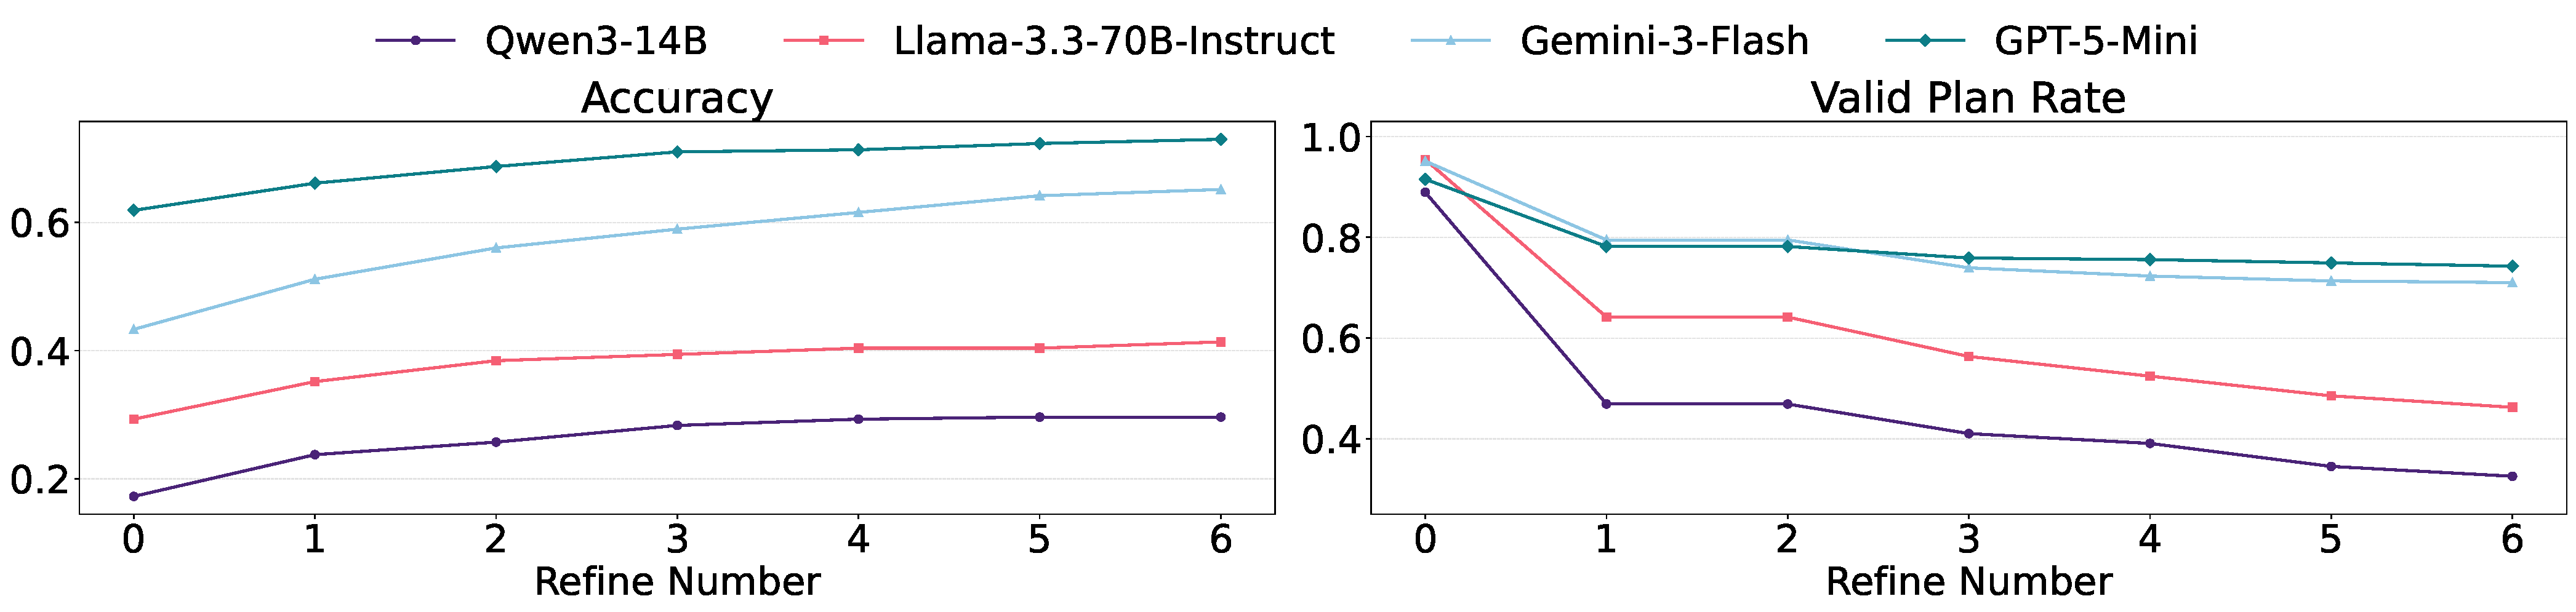
\includegraphics[width=\linewidth]{figures/accuracy_valid_plan_rate_refinednewx.pdf}
    \vspace{-0.25in}
    \caption{Model performance under $\mathcal{E}_{mid}$ with rubric-based refinement. Additional feedback yields only modest recovery and often destabilizes planning.}
    \label{fig:analysis-rubrics-refinement}
    \vspace{-0.17in}
\end{figure*}



If making prior constraints explicit is insufficient to recover performance, we next ask whether feedback on failed planning dimensions can help the model revise its plan. 
To test this, we conduct a refinement analysis in which, for failed queries (i.e., cases with neither early stopping nor success), the model is given feedback on unsatisfied rubric dimensions and allowed to revise its plan (details in Appendix~\ref{app:refine-rubrics-analysis-details}).
As shown in Figure~\ref{fig:analysis-rubrics-refinement}, we allow 1--6 additional refinement turns and evaluate performance after each turn. 
Accuracy improves only modestly, by around 10\%, whereas VPR drops sharply, by roughly 40\% for the two open-source models and 20\% for the two proprietary models.
This suggests that rubric feedback can correct some local planning errors, but often at the cost of violating constraints that were previously satisfied. 
One possible explanation is that models exhibit a recency-biased adaptation pattern: when receiving new rubric-level feedback, they tend to prioritize repairing the newly identified weakness rather than preserving consistency with all previously disclosed constraints.
Thus, refinement guidance can improve some local rubric dimensions, but it does not reliably support globally consistent plan revision under accumulated constraints, and can substantially undermine constraint validity.


\paragraph{User constraints contribute disproportionate difficulty.}
Since these corrective signals do not resolve the degradation, we next ask which constraints drive this difficulty. 
To isolate their effects, we perform a dual-ablation study with three conditions, \textit{World-Constraint Only}, \textit{User-Constraint Only}, and \textit{Both Constraints}, and evaluate each condition using accuracy and VPR.
As shown in Figure~\ref{fig:analysis-dual-ablation}, the pattern is clear across models: among the single-sided settings, \textit{User-Constraint Only} is consistently harder than \textit{World-Constraint Only}, while \textit{Both Constraints} is the most demanding setting.
This pattern suggests that user constraints contribute disproportionate difficulty in the dual-constraint setting and are a major source of planning instability. 
One possible reason is that user constraints often impose broader restrictions on the feasible action space: a single user preference may rule out many tools, actions, or modes of tool use, even when it appears as only one explicit constraint.

% \begin{figure*}[t]
% \centering
%     \begin{minipage}{0.5\textwidth}
%         \centering
%         \includegraphics[width=\textwidth]{figures/accuracy_dual_ablation.pdf}
%     \end{minipage}%
%     \hfill
%     \begin{minipage}{0.5\textwidth}
%         \centering
%         \includegraphics[width=\textwidth]{figures/valid_plan_rate_dual_ablation_normalize.pdf}
%     \end{minipage}
%     \vspace{-0.12in}
%     \caption{Model performance under different constraint sources. User constraints cause larger degradation than world constraints, and the full dual-constraint setting is the most challenging overall.}
%     \label{fig:analysis-dual-ablation}
%     \vspace{-0.1in}
% \end{figure*}

\begin{figure*}[t]
% \vspace{-0.5in}
    \centering
    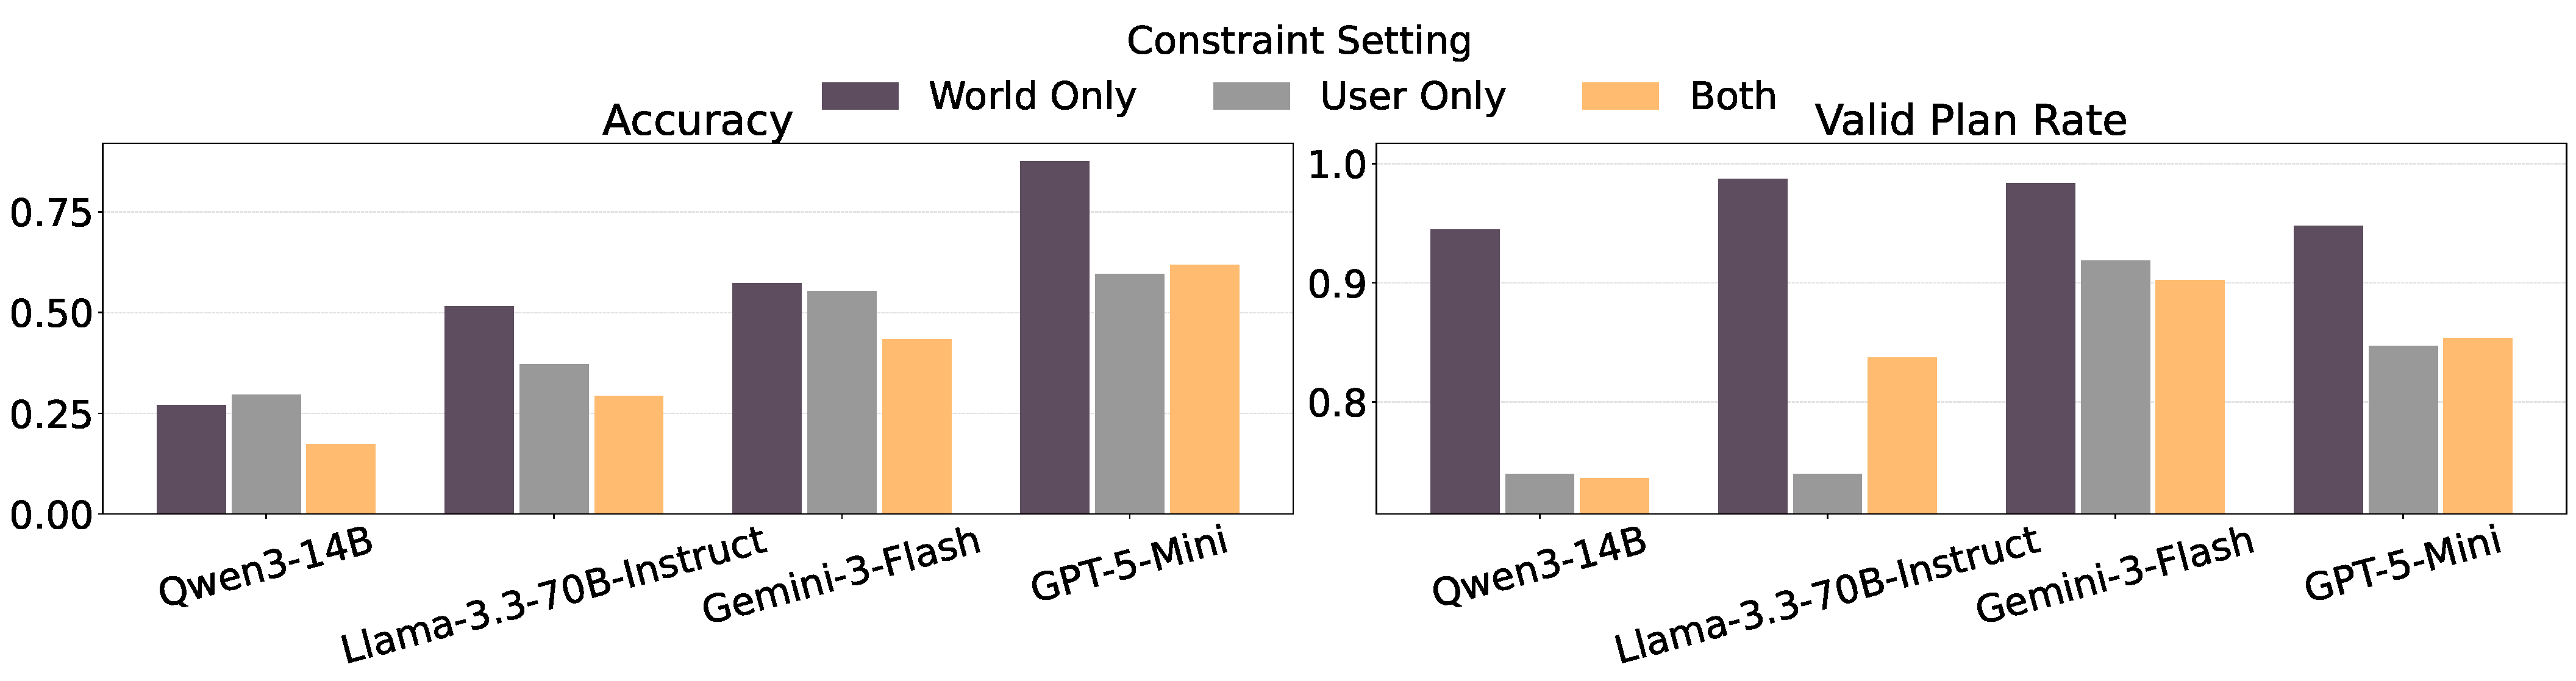
\includegraphics[width=\linewidth]{figures/accuracy_valid_plan_rate_dual_ablation.pdf}
    \vspace{-0.2in}
    \caption{Model performance under $\mathcal{E}_{mid}$ across constraint sources. User constraints cause larger degradation than world constraints, and dual-constraint setting is the hardest.}
    \label{fig:analysis-dual-ablation}
    \vspace{-0.2in}
\end{figure*}

% \begin{table*}[t]
% \centering
% \small
% \setlength{\tabcolsep}{2pt}
% \setlength{\extrarowheight}{2pt}
% \resizebox{\linewidth}{!}{
% \begin{tabular}{lcccccccc}
% \toprule
% Model & Feasibility & Physical & Ordering & Effectiveness & Concreteness & Safety & Consequence & Autonomy \\
% \midrule
% Qwen3-8B & \textbf{4.859} & 3.537 & 4.470 & 3.176 & 4.355 & 4.411 & 3.128 & 4.974 \\
% Qwen3-14B & 4.845 & 3.341 & 4.382 & 2.880 & 4.356 & 4.464 & 3.032 & 4.946 \\
% Qwen3-32B & \underline{4.854} & 3.774 & 4.660 & 3.416 & 4.720 & 4.558 & 3.392 & 4.961 \\
% Llama-3.3-70B-Instruct & 4.639 & 3.736 & 4.522 & 2.966 & 3.897 & 4.576 & 3.330 & 4.874 \\
% DeepSeek-V3.2 & 4.691 & 3.992 & 4.757 & 3.203 & 4.676 & 4.498 & 3.268 & 4.885 \\
% gemini-3-flash & 4.510 & 4.191 & 4.855 & 3.971 & 4.921 & 4.460 & 3.704 & 4.977 \\
% gemini-3.1-pro & 4.295 & 4.039 & 4.838 & 3.864 & \underline{4.955} & 4.506 & 3.687 & \textbf{4.986} \\
% gpt-5 & 4.366 & \underline{4.559} & \underline{4.911} & \underline{4.309} & 4.942 & \underline{4.825} & \underline{4.474} & \underline{4.984} \\
% gpt-5-mini & 4.592 & \textbf{4.601} & \textbf{4.922} & \textbf{4.329} & \textbf{4.967} & \textbf{4.857} & \textbf{4.686} & 4.970 \\
% gpt-5-nano & 4.465 & 4.310 & 4.765 & 3.712 & 4.660 & 4.824 & 4.230 & 4.796 \\
% \bottomrule
% \end{tabular}
% }
% \caption{Turn-wise analysis: final-turn rubric means.}
% \label{tab:turnwise-final}
% \vspace{-0.2in}
% \end{table*}








\begin{takeaway}
\label{sec:error-analysis}
\textbf{Error Analysis: }
Model failures primarily manifest as degraded task effectiveness and weak physical grounding under accumulated dual constraints.
\end{takeaway}


% \jiayu{Insert in the Table!!}

\paragraph{Task effectiveness degrades under accumulated dual constraints.}
As shown in Table~\ref{tab:turnwise-final-selected}, \textit{Effectiveness} is consistently one of the weakest dimensions across models. 
This weakness also becomes more pronounced over interaction, as Figure~\ref{fig:analysis-turnwise} shows a clear decline across turns and especially poor performance in the final stage. 
This trend suggests that current models struggle to maintain an effective plan under extended, constraint-heavy interaction.


\paragraph{Physical grounding remains weak under accumulated dual constraints.}
Table~\ref{tab:turnwise-final-selected} also shows consistently weak performance in \textbf{Physical} grounding. 
This suggests that models often fail to reason adequately about the physical consequences of their tool use under progressively disclosed constraints. 
As a result, their plans may appear coherent overall, while still overlooking key physical conditions such as object accessibility or spatial compatibility.
We provide more detailed examples in Appendix~\ref{app:error-example}.

